\section{\label{sec:resonances}Comparison of Data to Known States and Cross Sections}

In this section we show a series of figures depicting known resonances with the \abbr{g12} data. The reader is encouraged to compare the masses and widths measured with the PDG\cite{pdg}. The masses of the narrow states in g12 are all measured to be consistent with the known values, such as η in Fig.~\ref{fig:resonances.eta} using the missing mass technique, π$^0$ reconstructed using two photons Fig.~\ref{fig:resonances.2gamma.pi0}, ρ/ω reconstructed using two leptons Fig.~\ref{fig:resonances.ee.rho_omega}, as well as Ξ$^-$ from the reaction of γ π $\rightarrow$ K$^+$ K$^+$ ($X$) shown in Fig.~\ref{fig:resonances.xi}. \begin{v2}Fig.~\ref{fig:resonances.kstar} shows the invariant mass of the K$^*$ from K$^+$ [π$^0$]. In addition to these missing masses, we have already shown a good $K_s$ signal from π$^+$ π$^-$ in Fig.~\ref{fig:beamcor.k_mass} on page~\pageref{fig:beamcor.k_mass}. The $K^{*+}$, shown in Fig.~\ref{fig:resonances.kstar}, and the $\phi(1020$ shown in Fig.~\ref{fig:resonances.phi}, are also spot on when compared with the PDG values.\end{v2}

\begin{figure}[htpb]\begin{center}
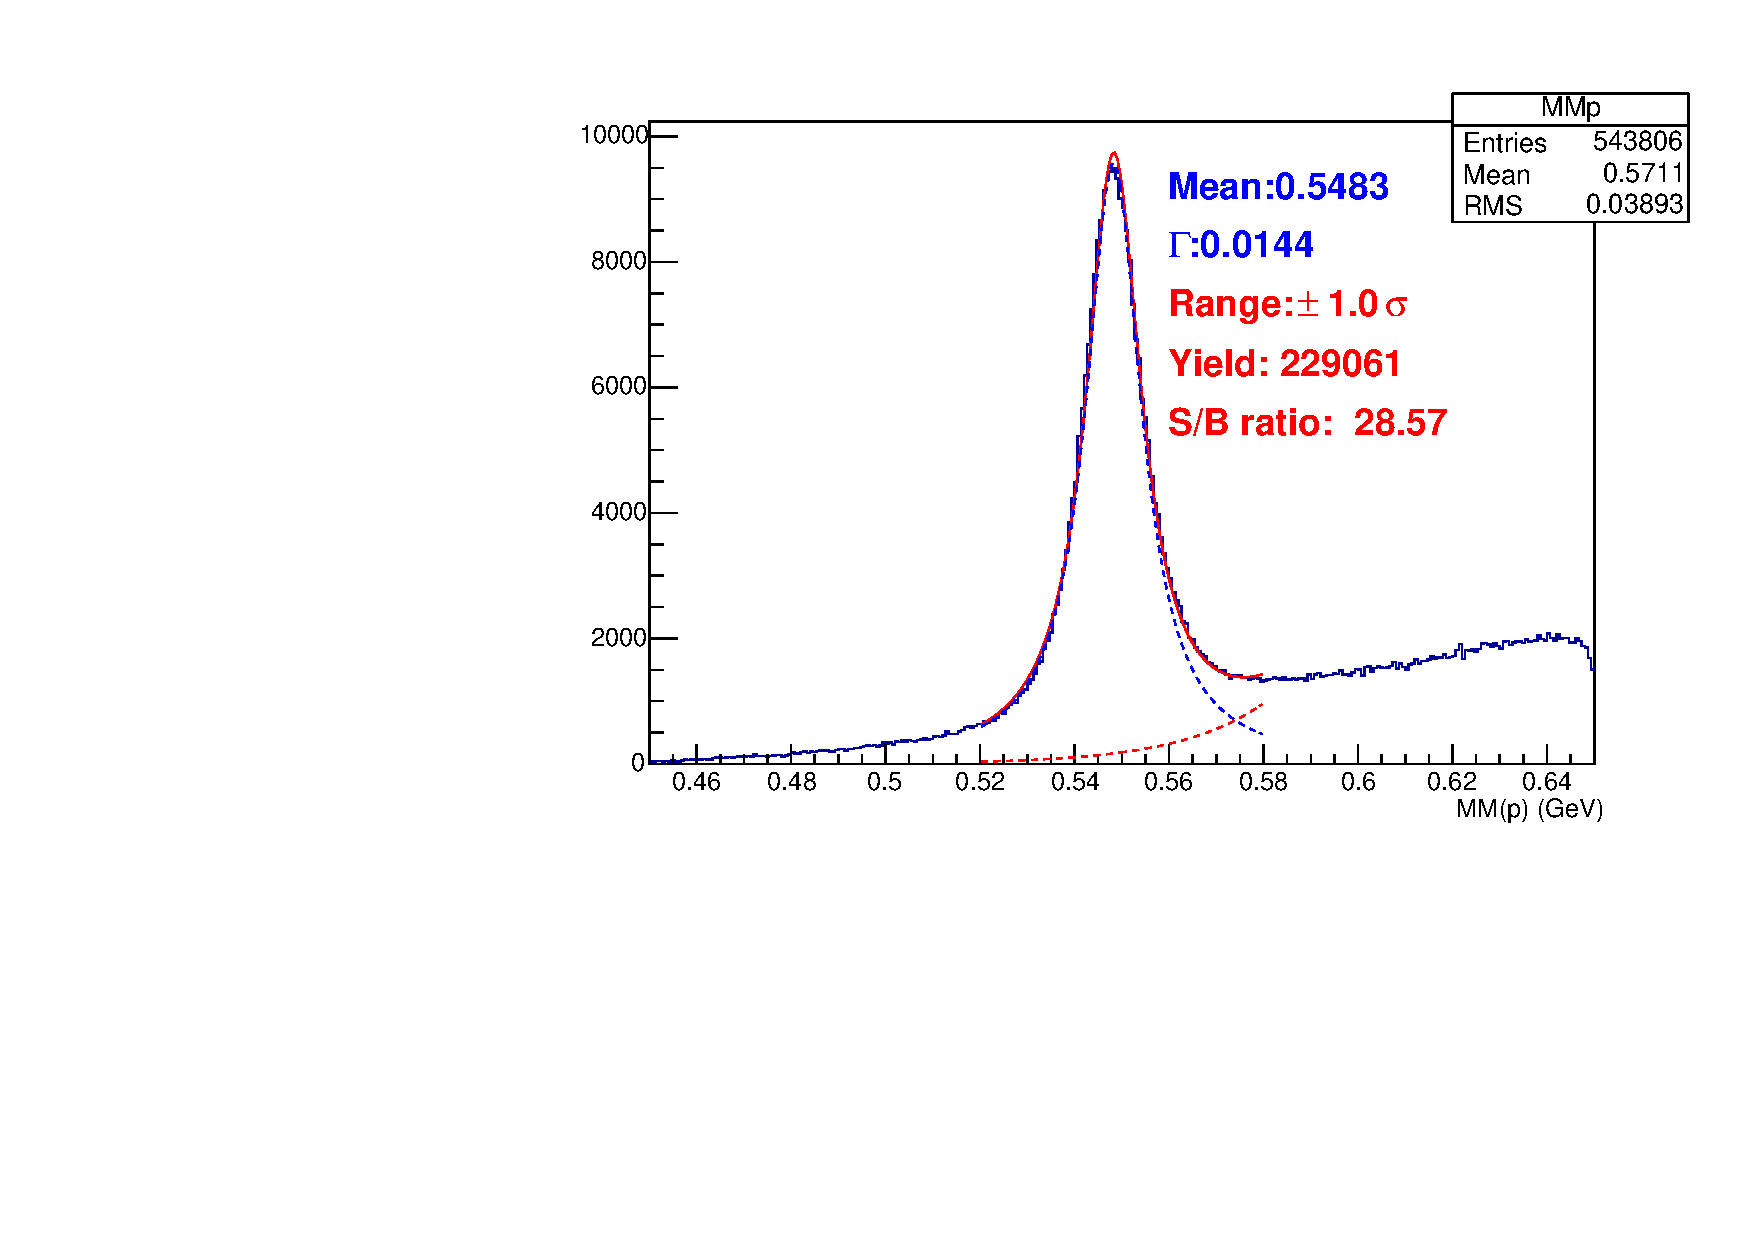
\includegraphics[width=0.4\columnwidth,angle=-90]{{figures/resonances/MMp-eta}.pdf}
\caption[]{\label{fig:resonances.eta}Missing mass off proton showing the η resonance with a measured mass of 548~MeV.}
\end{center}\end{figure}

\begin{figure}[htpb]\begin{center}
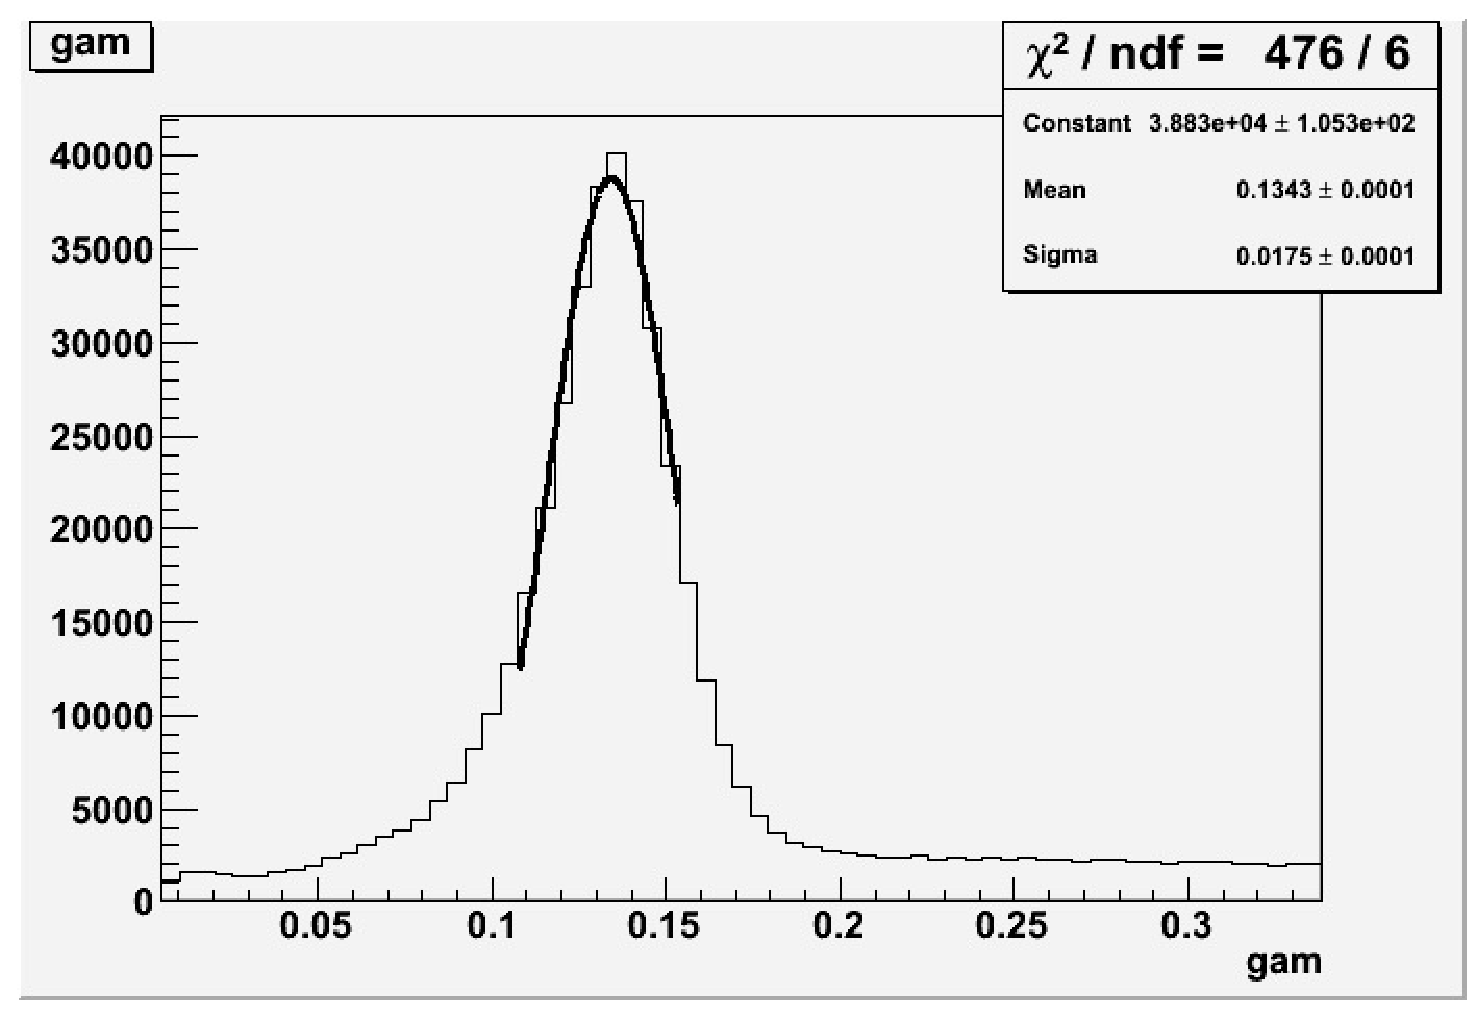
\includegraphics[width=0.4\columnwidth]{{figures/resonances/2gamma-pi0-p2pi2g}.eps}
\caption[]{\label{fig:resonances.2gamma.pi0}Invariant mass of two final-state photons showing the π$^0$ meson.}
\end{center}\end{figure}

\begin{figure}[htpb]\begin{center}
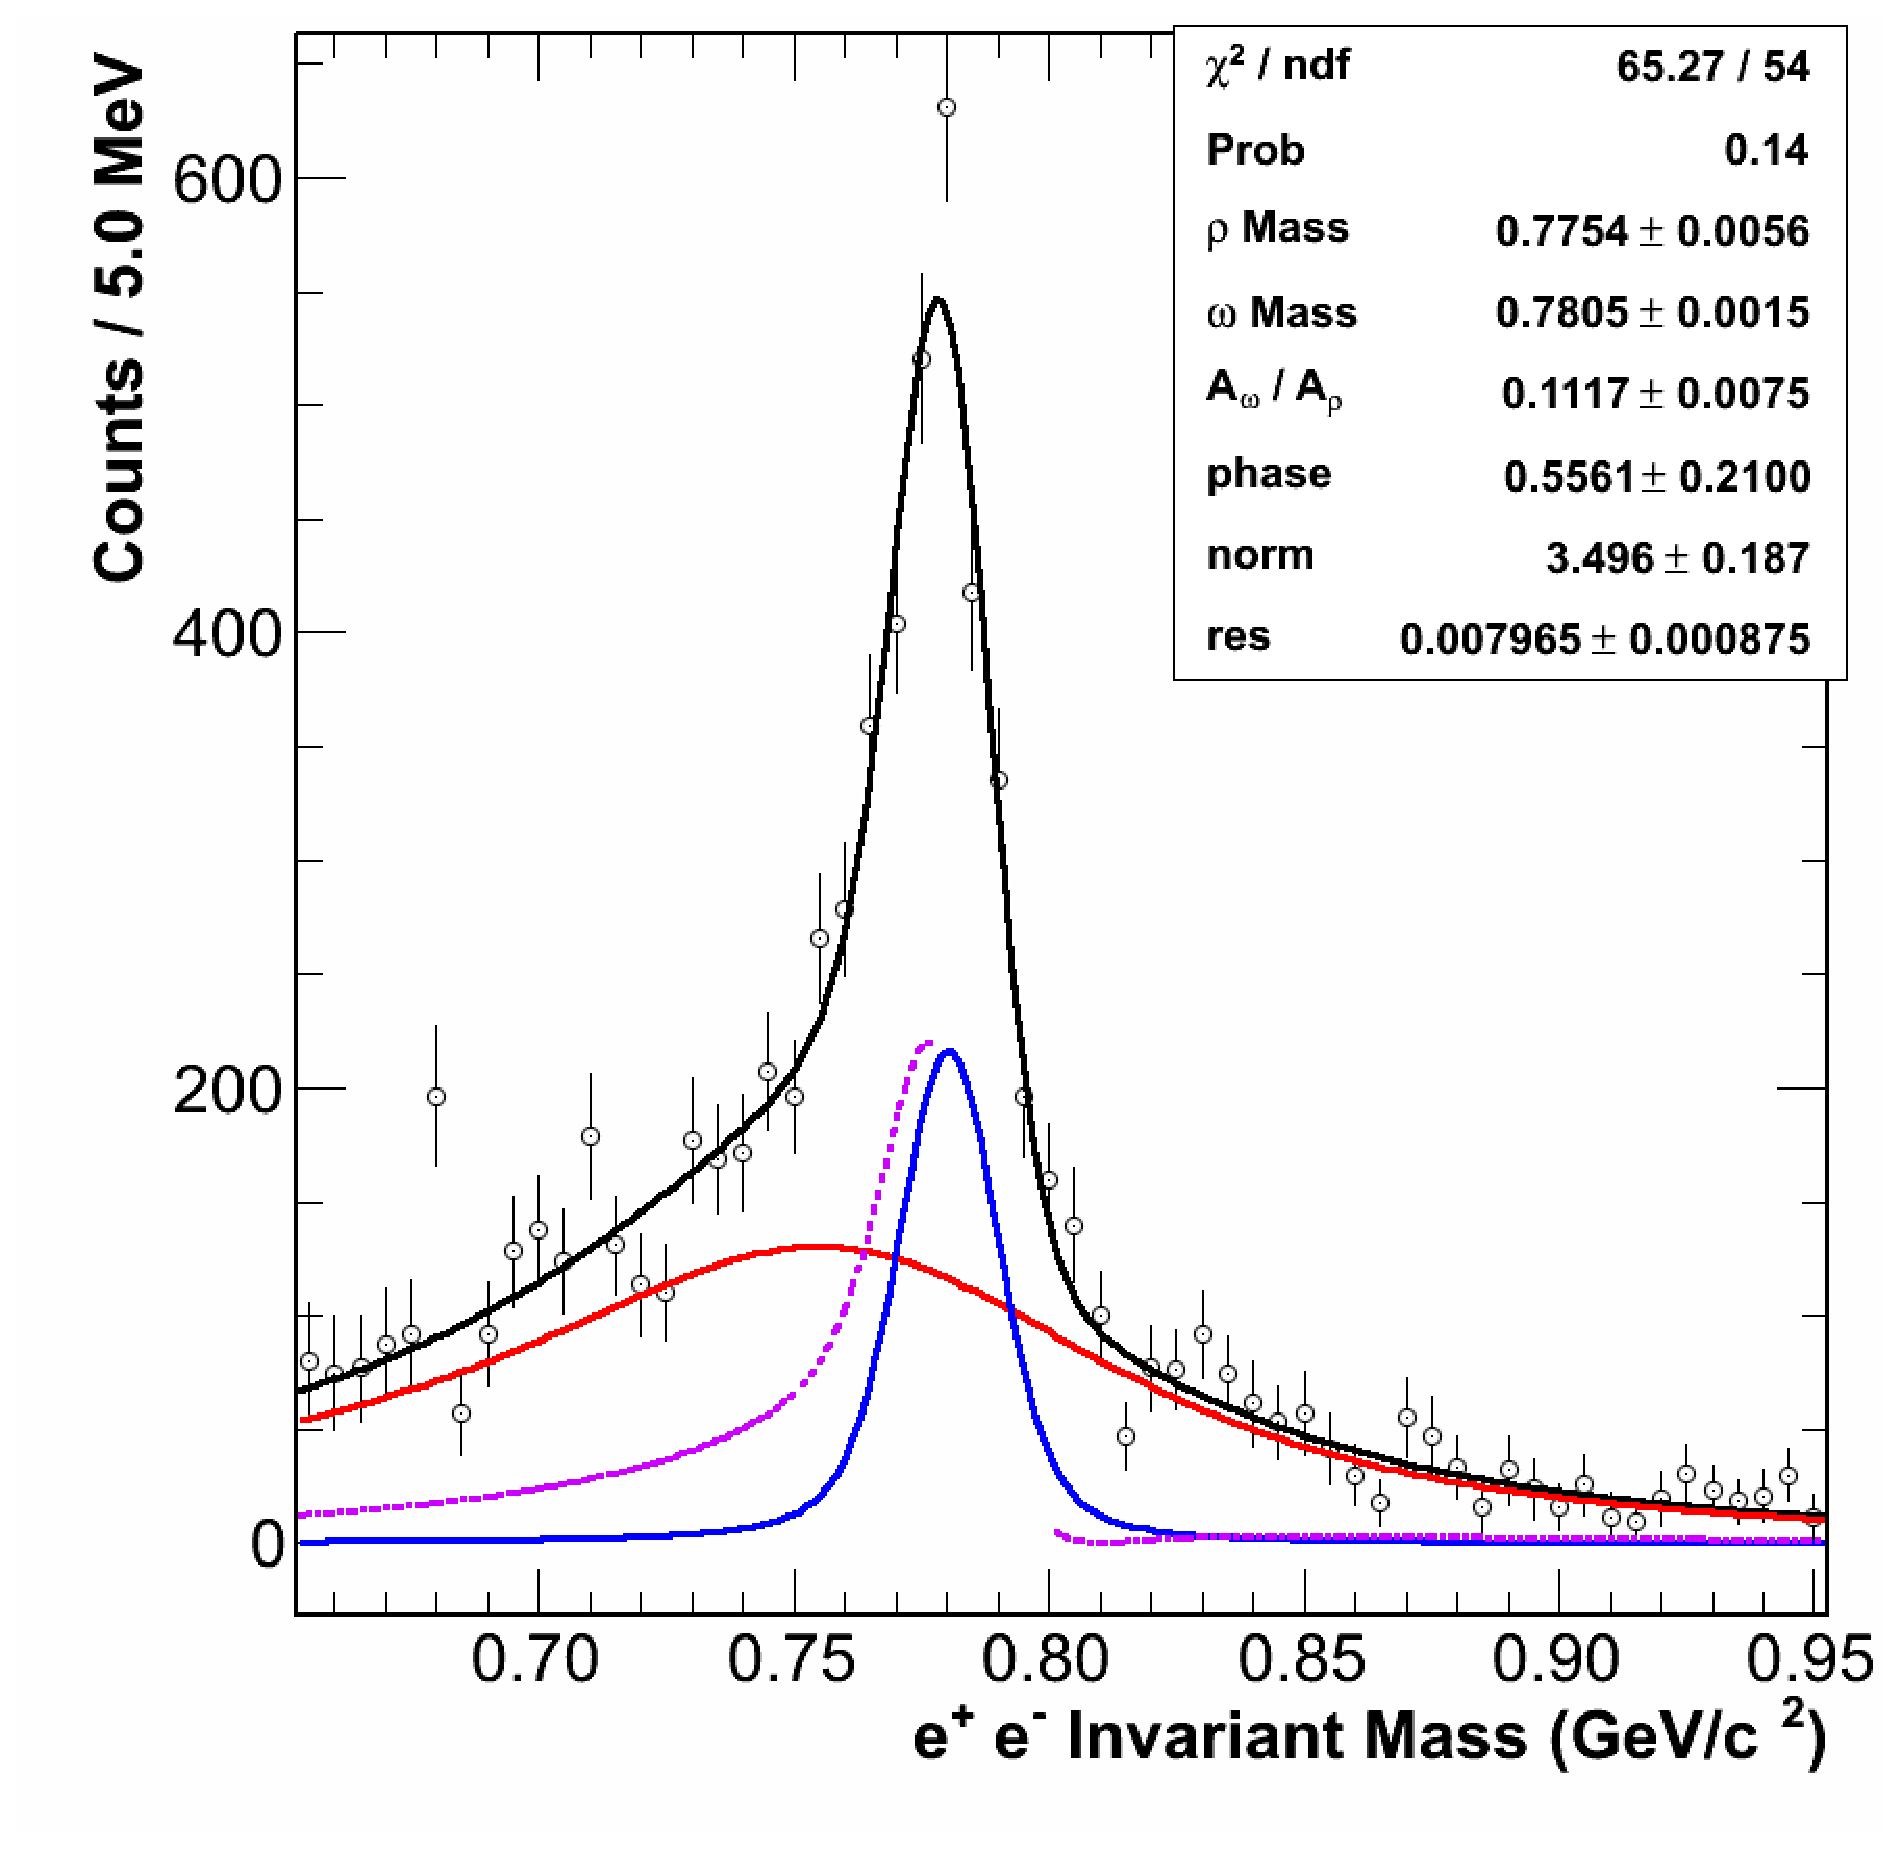
\includegraphics[width=0.4\columnwidth]{{figures/resonances/Sys_NormalRange}.eps}
\caption[]{\label{fig:resonances.ee.rho_omega}Invariant mass of electron and positron pair showing the (mixed) ρ and ω mesons.}
\end{center}\end{figure}

\begin{figure}[htpb]\begin{center}
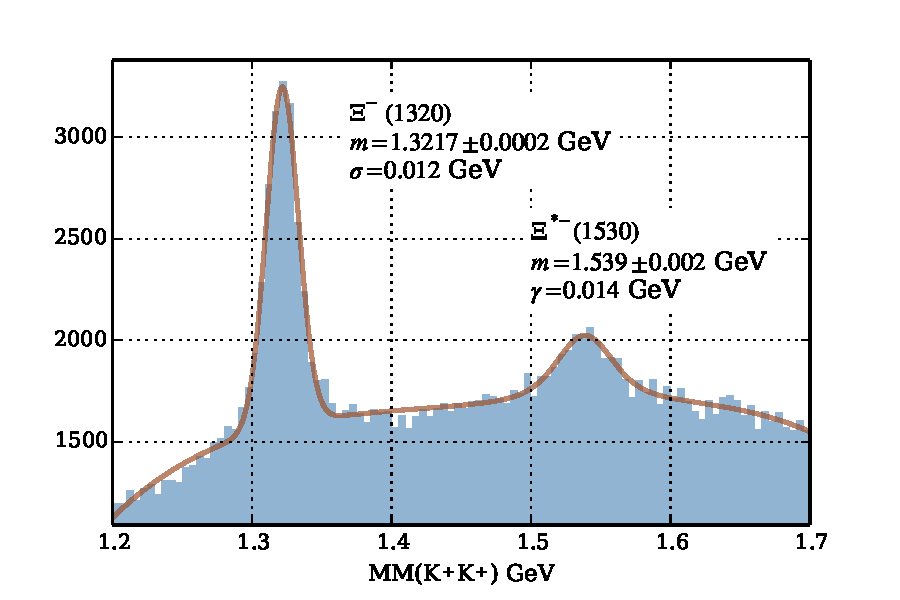
\includegraphics[width=0.4\columnwidth]{{figures/resonances/g12_mmkk_xisignals}.pdf}
\caption[]{\label{fig:resonances.xi}Missing mass off K$^+$K$^+$ showing the ground state and first-excited Ξ$^-$ resonances. The ground state is fit to a Gaussian with a width shown as $σ$, while the first excited state is fit to a Voigtian with a (scaled) Gaussian width taken from the ground state. The value $γ$ shown is the Lorentzian width of the fit.}
\end{center}\end{figure}

\begin{figure}[htpb]\begin{center}
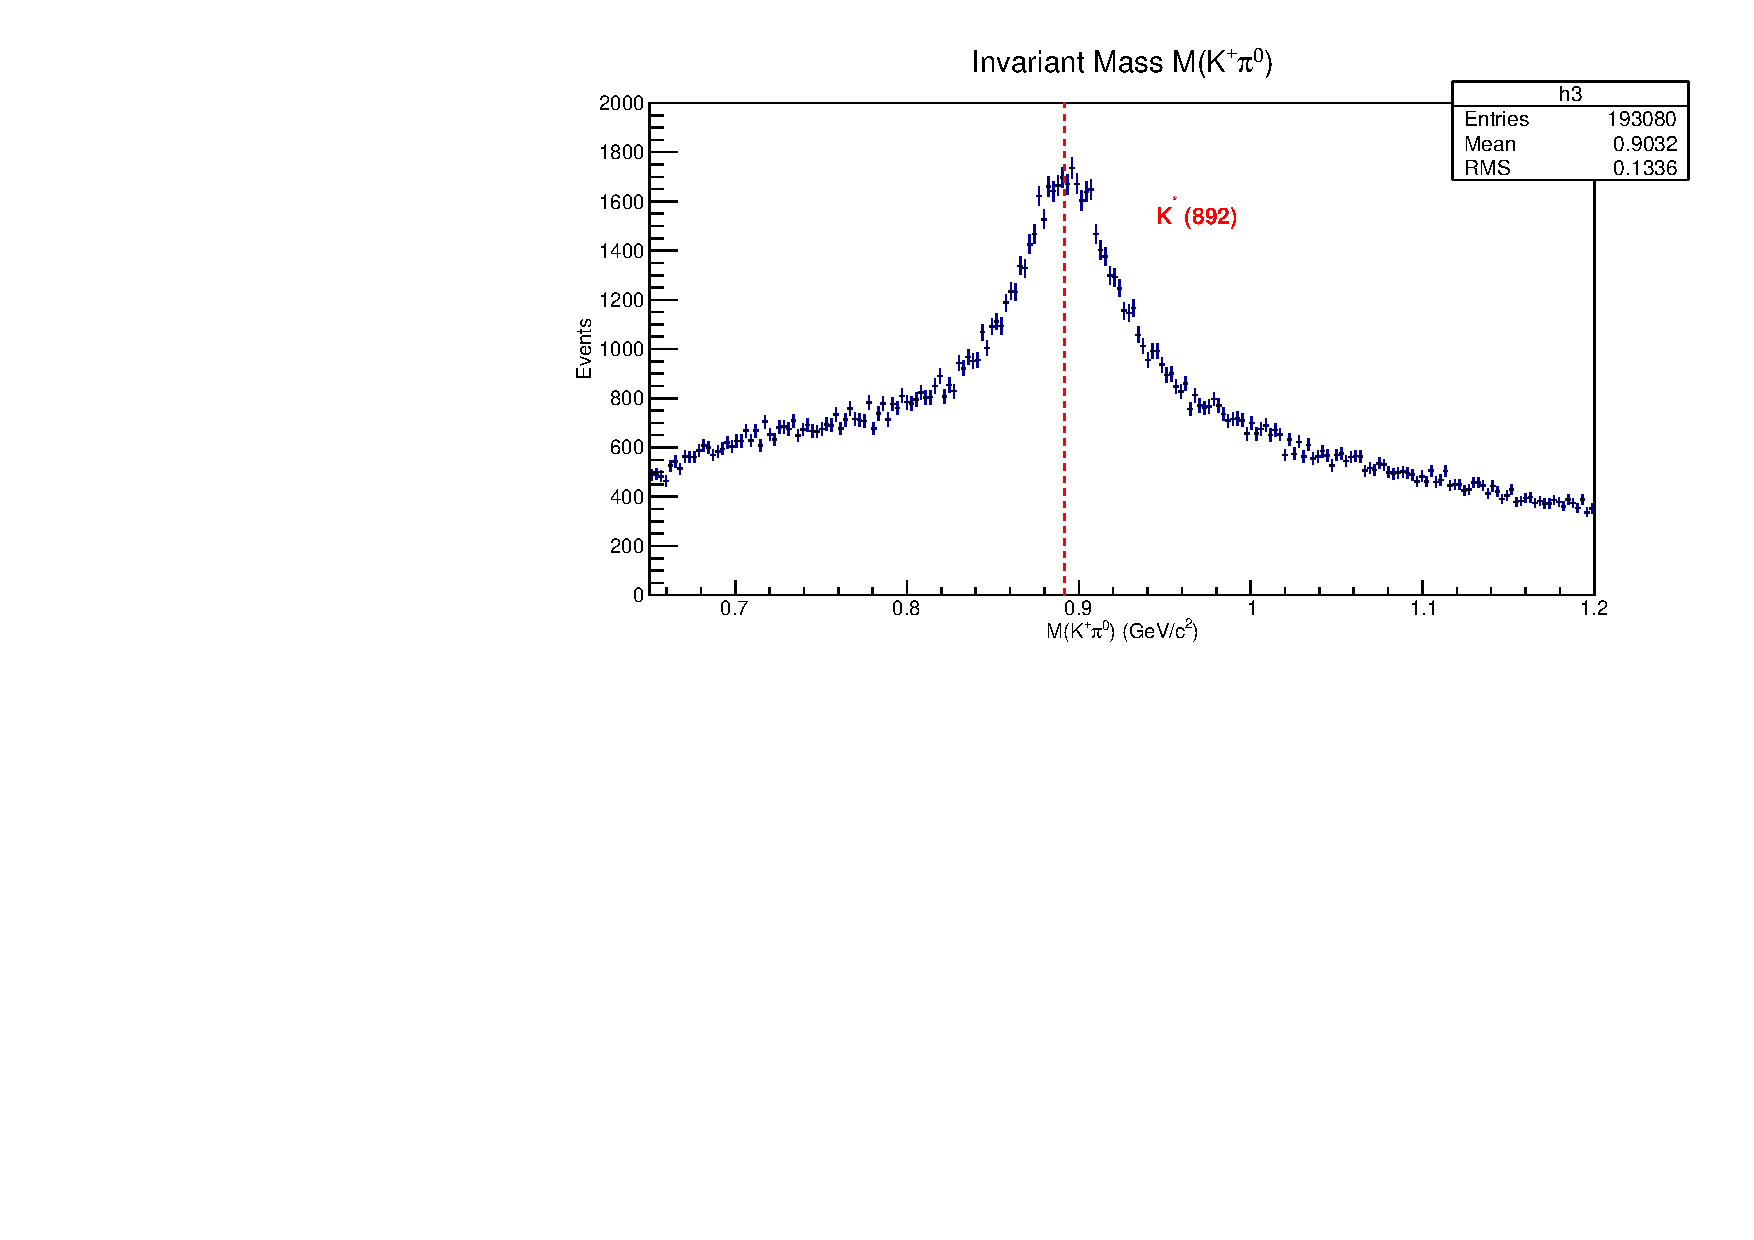
\includegraphics[width=0.4\columnwidth,angle=270]{{figures/resonances/kstar_err}.pdf}
\caption[K$^*$ Mass]{\label{fig:resonances.kstar} K$^+$ [π$^0$] invariant mass spectrum in the reaction $\gamma p \rightarrow K^+ \Lambda (\pi^0)$, where $\pi^0$ was constrained to the PDG mass. The line indicates the PDG value of $K^{*+}$ mass. $\Lambda \rightarrow p\pi^-$ events are selected.}
\end{center}\end{figure}
\begin{v2}
\begin{figure}[htpb]\begin{center}
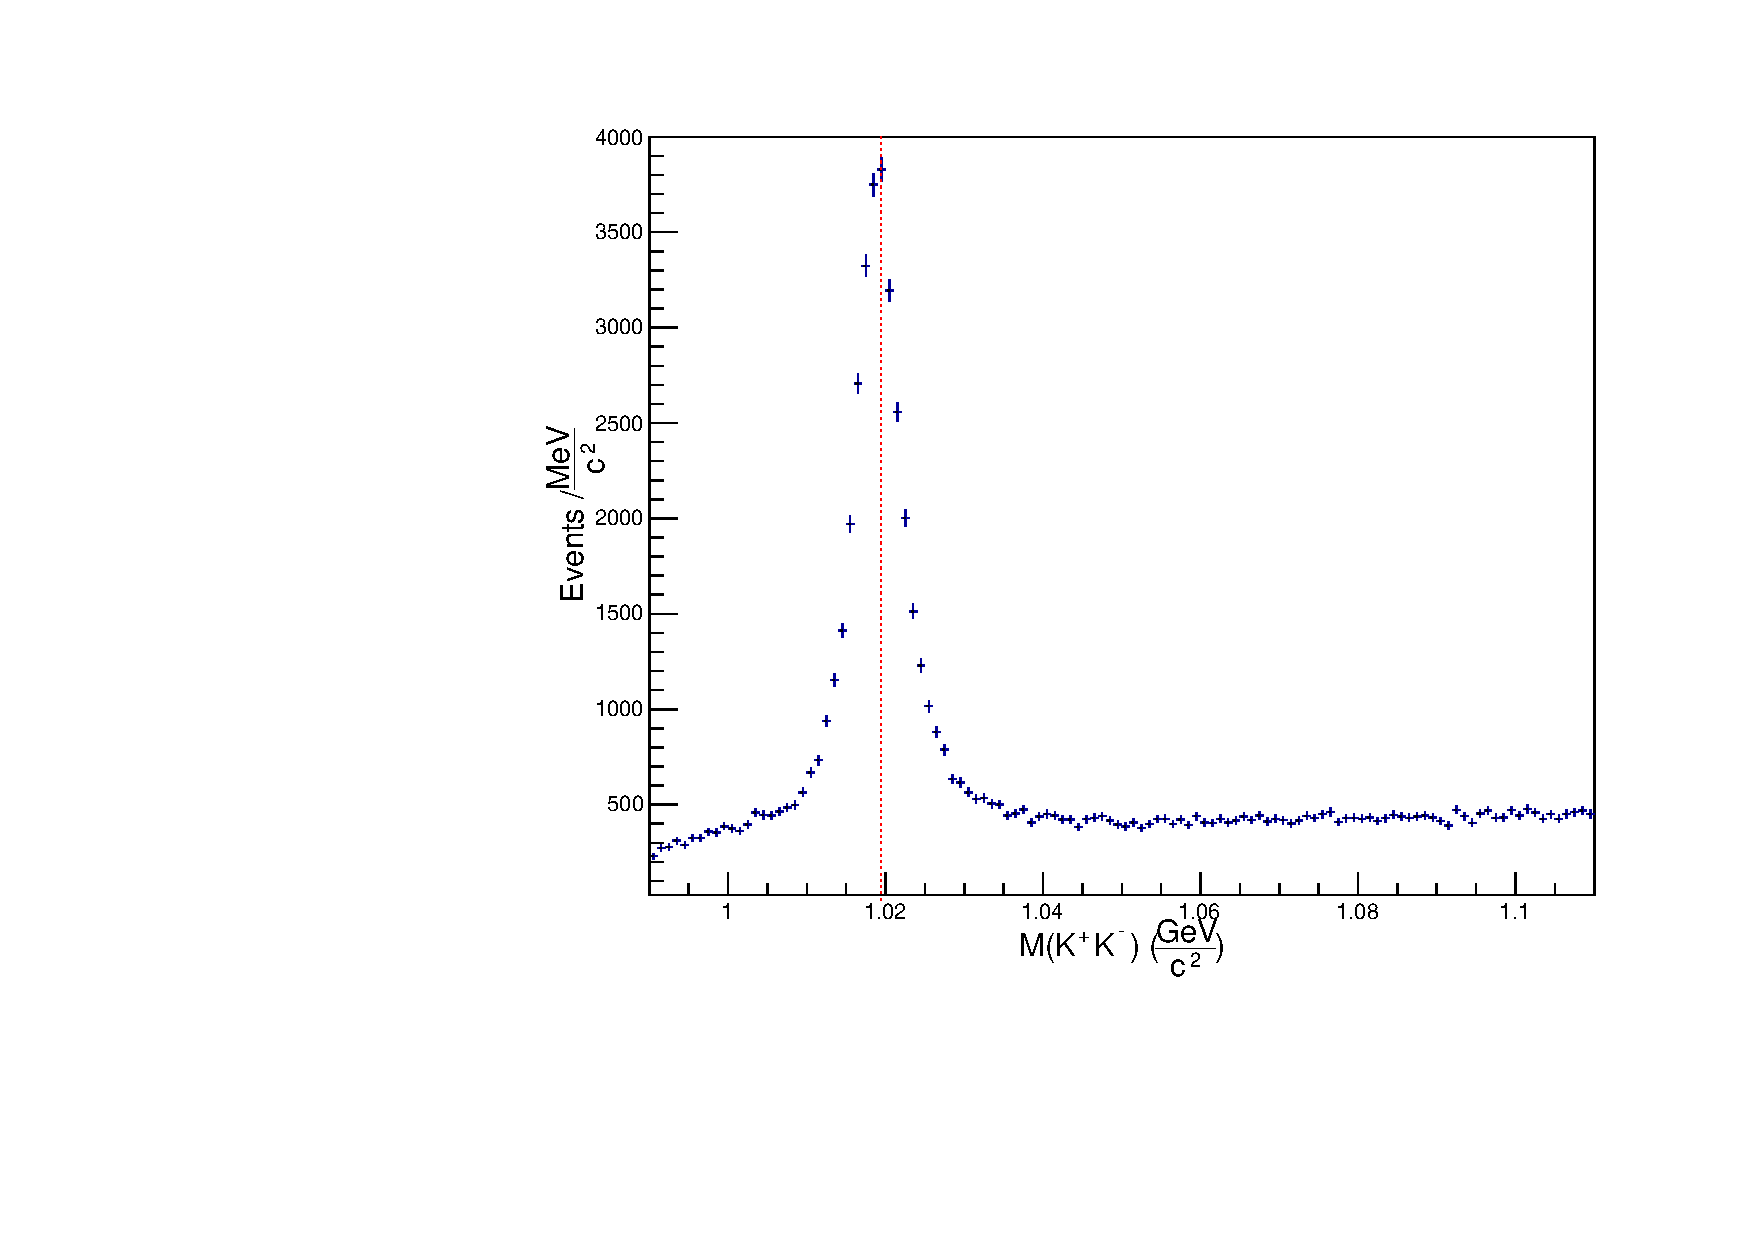
\includegraphics[width=0.4\columnwidth,angle=270]{{figures/resonances/phi_IM_kk}.pdf}
\caption[KK Mass]{\label{fig:resonances.phi}$K^+K^-$ invariant mass spectrum in the reaction $\gamma p \rightarrow K^+ K^- p$, where all particles are detected by CLAS. The line indicates the PDG value of $\phi(1020)$ mass.}
\end{center}\end{figure}



\subsection{\label{sec:trackEff}Track dependent inefficiency correction}
If the efficiencies of the detectors and the triggers have been measured and modeled perfectly, then it's reasonable to expect that the reconstruction efficiency can be faithfully reproduced in simulation on a track-by-track basis. For the charged particles, this has been investigated thoroughly using the reaction $\gamma p \rightarrow p \pi^+ \pi^-$ events, using the  ollowing 3 topologies:
\begin{align}\label{eq:eff_topologies}
\gamma p \rightarrow p \pi^+ (\pi^-) \nonumber\\
\gamma p \rightarrow p \pi^- (\pi^+)  \nonumber\\
\gamma p \rightarrow \pi^+ \pi^- (p)
\end{align}

The efficiency map was derived for each particle, as a function of momentum, angles ($\theta, \phi$) in the lab frames, as well as the vertex positions, in the same manner for $p, \pi^+, \pi^-$. The results of pions can be applied to kaons for analyses involving detected kaons. For example, for $\pi^+$, the reconstruction efficiency can be derived using the $ \gamma p \rightarrow p \pi^- (\pi^+)$. If $\pi^+$ can be can be reconstructed using the missing mass techniques and also pass the kinematic fitting probability cut $>1 \%$, then the data was checked to see if the $\pi^+$ was actually detected. This was done exactly the same way in both simulation and real data. In a perfect world, the ratio of the two efficiency map (Simulation devided by the real data) should be exactly $1$ everywhere. However, as can be seen in  Fig.~\ref{fig:PipEff}, the ratio is usually larger than $1$, indicating the simulation has an over efficiency on the order of $5 \%$. Similar over efficiency can also be seen for the $\pi^-$ and the proton, as shown in Fig.~\ref{fig:PimEff} and ~\ref{fig:ProtonEff}. For a final state that requires three charged tracks, this will lead to an correction that is on average about $18 \%$ globally. This correction accidentally is very similar to the g11 global normalization correction factor. However, the g12 correction is a function of momentum, angles and vertex positions, and is applied dynamically on a event-by-event basis. The standard g12 procedure for applying the above corrections can be applied using the routines found in the jlab SVN repository (\url{https://jlabsvn.jlab.org/svnroot}) here:
\begin{verbatim}
clas/users/mkunkel/clas/g12_corrections/g12_trackEfficiency.hpp
\end{verbatim}

\begin{figure}[htpb]\begin{center}
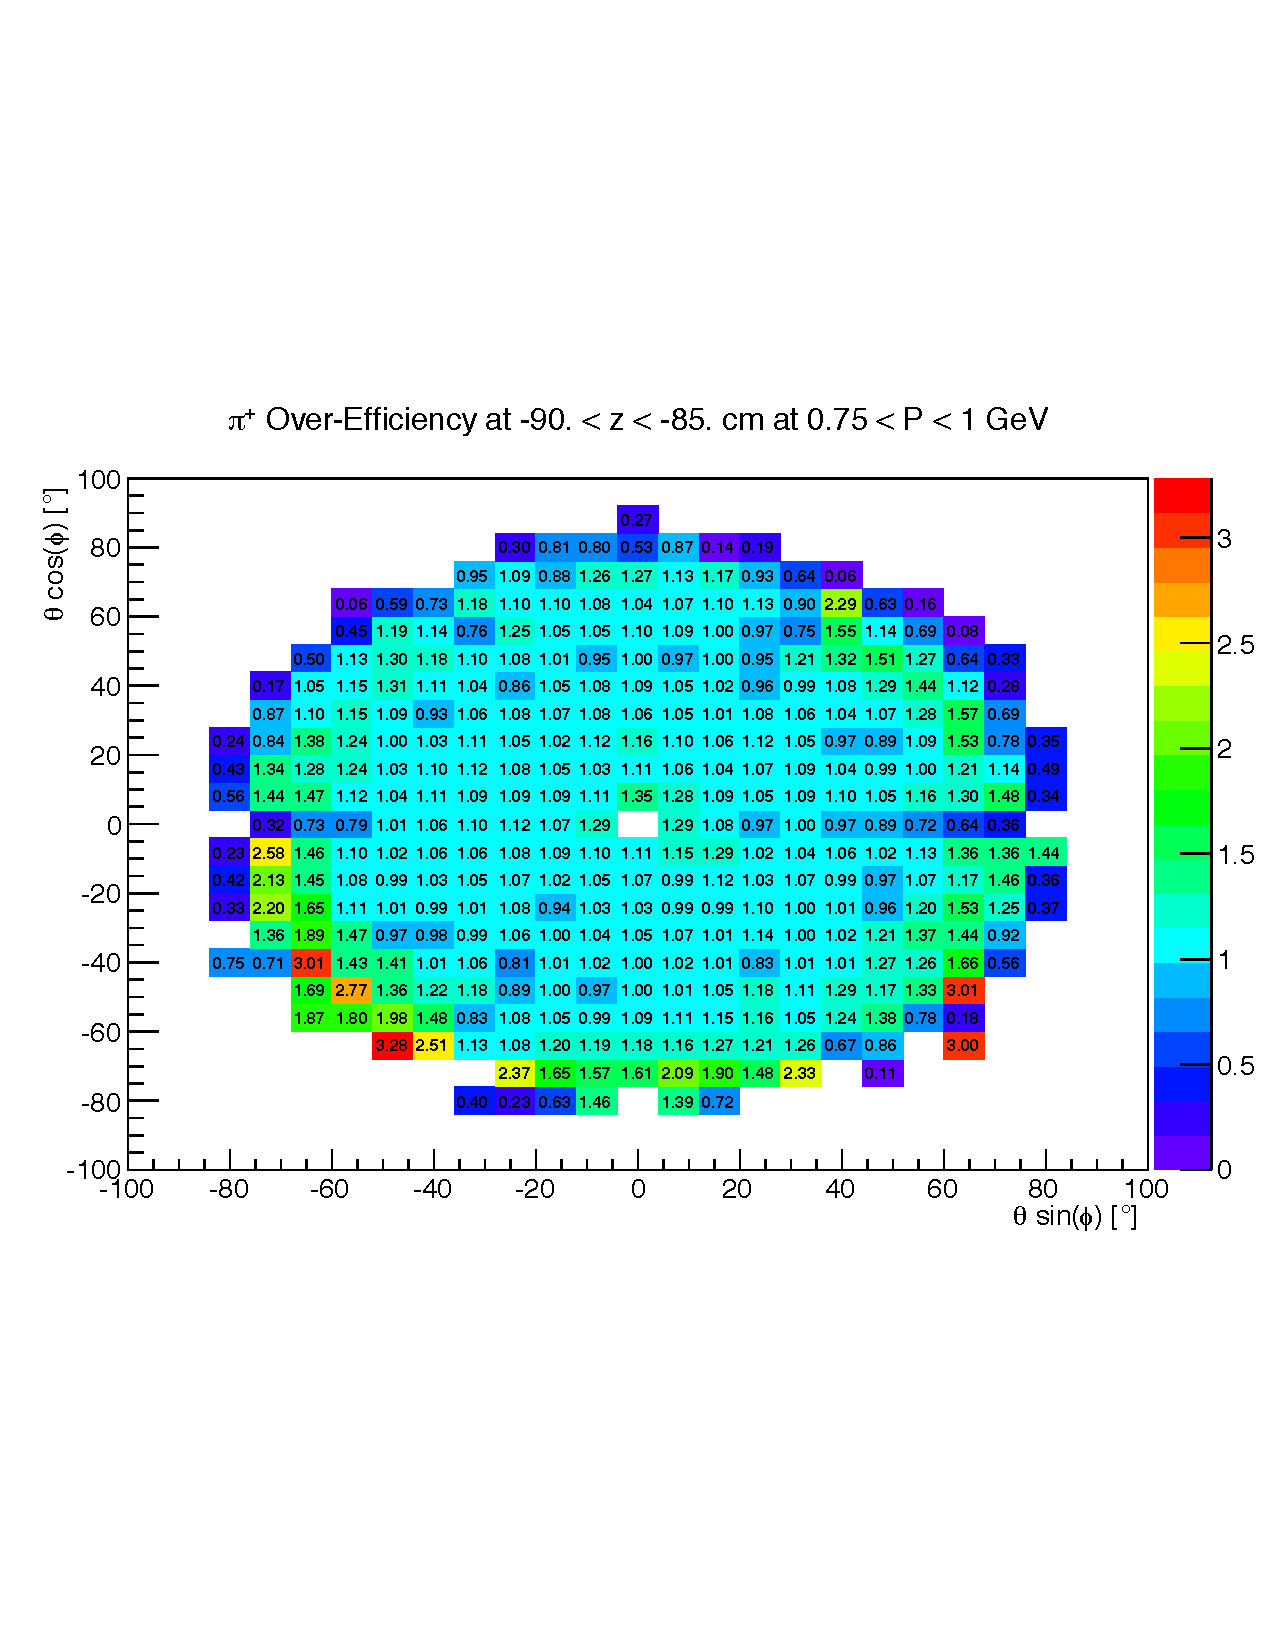
\includegraphics[width=1.1 \figwidth,height=\hfigheight]{figures/xsec/Pip_Eff.pdf}
\caption{\label{fig:PipEff} $\theta \cos\phi$ vs. $\theta \sin\phi$ plot showing the over-efficiency of simulating the π$^+$ with z-vertex $z \in [-90,-85]$~cm and momentum $p \in [0.75,1]$~GeV from a 2 charged track reaction.}
\end{center}\end{figure}


\begin{figure}[htpb]\begin{center}
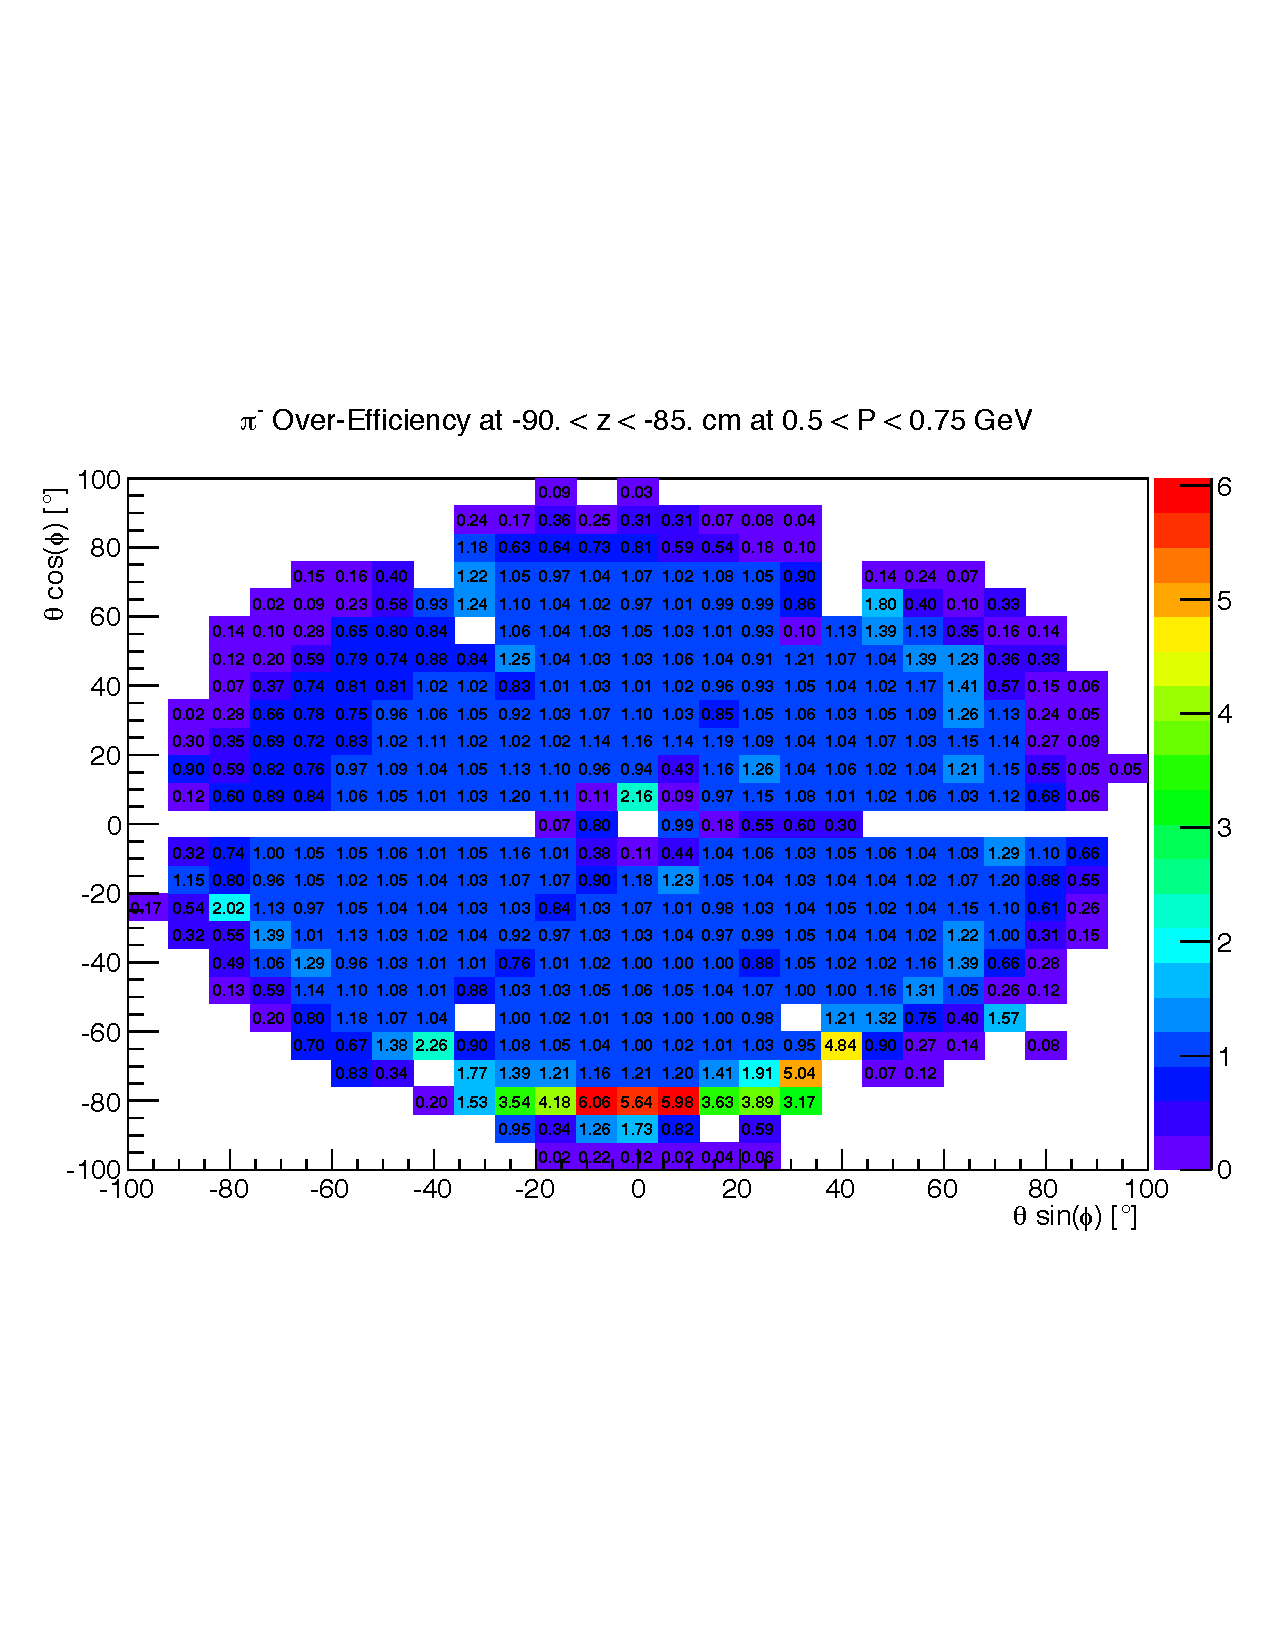
\includegraphics[width=1.1 \figwidth,height=\hfigheight]{figures/xsec/Pim_Eff.pdf}
\caption{\label{fig:PimEff} $\theta \cos\phi$ vs. $\theta \sin\phi$ plot showing the over-efficiency of simulating the $\pi^-$ with z-vertex $z \in [-90,-85]$~cm and momentum $p \in [0.75,1]$~GeV from a 2 charged track reaction.}
\end{center}\end{figure}

\begin{figure}[htpb]\begin{center}
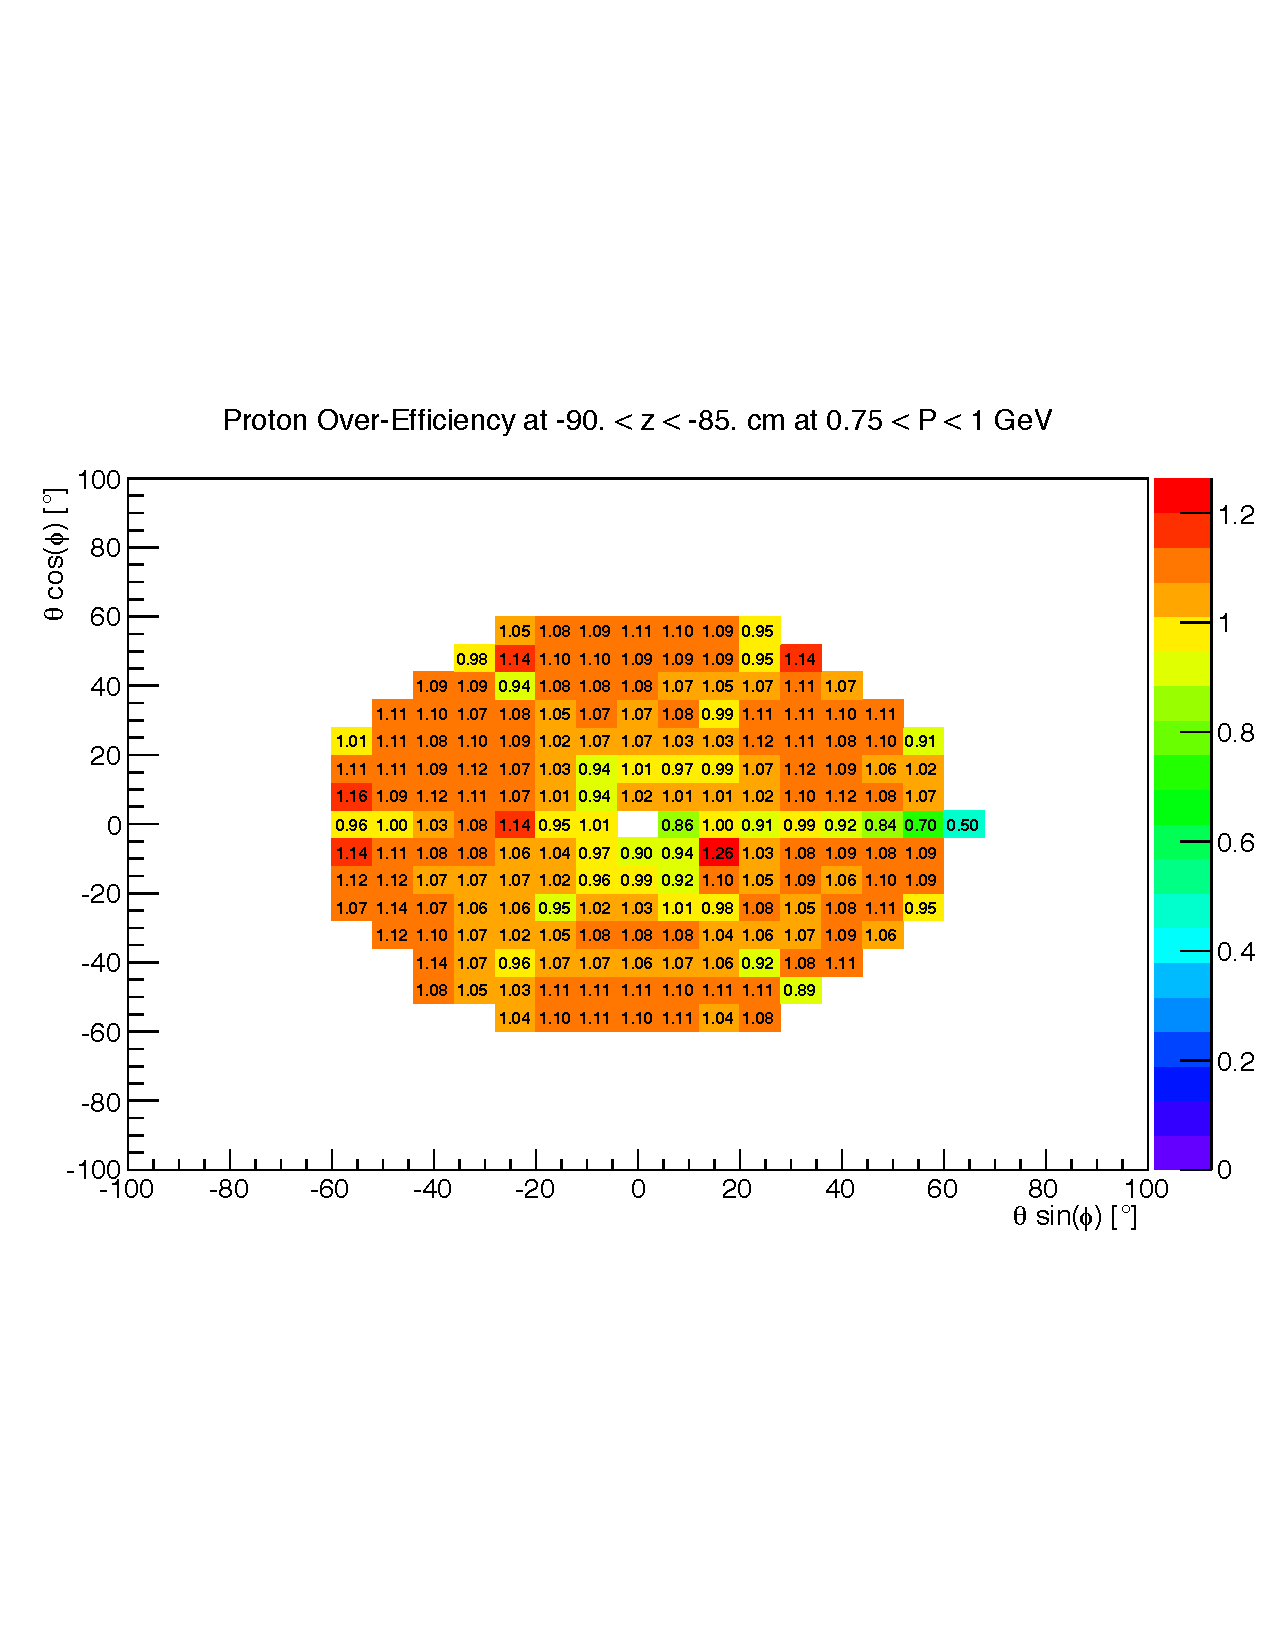
\includegraphics[width=1.1 \figwidth,height=\hfigheight]{figures/xsec/Proton_Eff.pdf}
\caption{\label{fig:ProtonEff} $\theta \cos\phi$ vs. $\theta \sin\phi$ plot showing the over-efficiency of simulating the proton with z-vertex $z \in [-90,-85]$~cm and momentum $p \in [0.75,1]$~GeV from a 2 charged track reaction.}
\end{center}\end{figure}


Further details about this procedure can be found in Reference~\cite{clas.thesis.kunkel}. It is important to point out that this track-dependent efficiency correction is also tied to the multiple photon correction, and can be derived by either accounting for  events lost to multiple photons, or using all photons in the chosen time bucket. The difference between this two methods can be used to be estimate the systematic uncertainty of this correction. For a three-charged tracks topology, the uncertainty is estimated to be around $3 \%$.
\end{v2}



\subsection{\label{sec:xsec}Comparison of Data to Known Cross Sections}

Various cross sections have been extracted using the g12 data set, all showing consistent results when compared with prior CLAS measurements if available, such as the ω, the Λ, as well as π$^0$. In particular, the ω cross section results(FSU) , measured using γ p $\rightarrow$ p π$^+$ π$^-$ (π$^0$), are presented here and compared with the g11 results and are consistent across the g12 photon energy range. Although some disagreements do show up at particular kinematic bins, it's safe to say that g12 does not have an overall normalization issue.

Figures~\ref{fig:xsec.omega1} and \ref{fig:xsec.omega2} show the differential cross sections for the reaction: γ p $\rightarrow$ p ω, based on the dominant decay mode: ω $\rightarrow$ π$^+$ π$^-$ π$^0$. For this analysis, we have selected events with two positively-charged tracks for the proton and the π$^+$ as well as one negatively-charged track for the π$^-$. The selection has used runs 56520 - 56572, 56573 - 56594, and 56608 - 56646 (Table~\ref{tab:data.trig.conf.2}), which were {\it event-sorted} according to {\bf 2-2pos1neg\_not\_1ckaon1ctrk} (Section~\ref{sec:data.pass1}). The analyzed run ranges comprise all g12-events that require in the trigger at least three charged tracks in three different sectors but were not subjected to {\it pre-scaling} to enhance events with high photon energies. This removed an additional layer of complication for studying normalization issues.

For the $\omega$ events, the standard {\sc eloss} corrections but tuned momentum corrections to the proper shape of the pull distributions in the kinematic fitting of the reaction: γ p $\rightarrow$ p π$^+$ π$^-$ (no missing particle). (For these particular results, the g12 beam energy correction is not applied) After all initial kinematic corrections, the three-track events were then subject to 1C kinematic fitting imposing energy and momentum conservation as well as requiring a missing π$^0$ in the reaction; events have then been selected with a confidence-level (CL) cut of 0.001 which essentially only demands fit convergence. In the final step, ω $\rightarrow$ π$^+$ π$^-$ π$^0$ events were identified in the invariant π$^+$ π$^-$ π$^0$ mass. The signal and background separation was achieved by applying the Q-value method which assigns a quality factor to each event indicating the likelihood for the event to be signal. The high efficiency of this method justifies the relatively small CL cut. At this point, we have not yet applied the fiduciary cuts discussed in this note. However, we do not expect any significant impact on our final results.

For the differential cross sections, the ω yields have been determined for 50-MeV wide energy bins and 20 bins in the corresponding angular distributions (of the ω in the overall center-of-mass system). Shown in Figs.~\ref{fig:xsec.omega1} and \ref{fig:xsec.omega2} is the energy range 1.50 - 3.80 GeV.  The angular distributions of the ω production were acceptance corrected by studying the reaction in GEANT-based simulations. These acceptance corrections include a simulation of the geometrical trigger configuration requiring three different tracks in three different sectors.  We have compared normalized and acceptance-corrected ω yields from the production runs (at 60 nA) as well as single-sector runs (at 24 nA) and observed a near perfect agreement over the full run range used in this analysis. From this we conclude that the current and trigger corrections are under control. The full energy range for the ω cross sections, obviously, will be discussed by the corresponding analysis note of this particular results by FSU.


\begin{figure}[htpb]\begin{center}
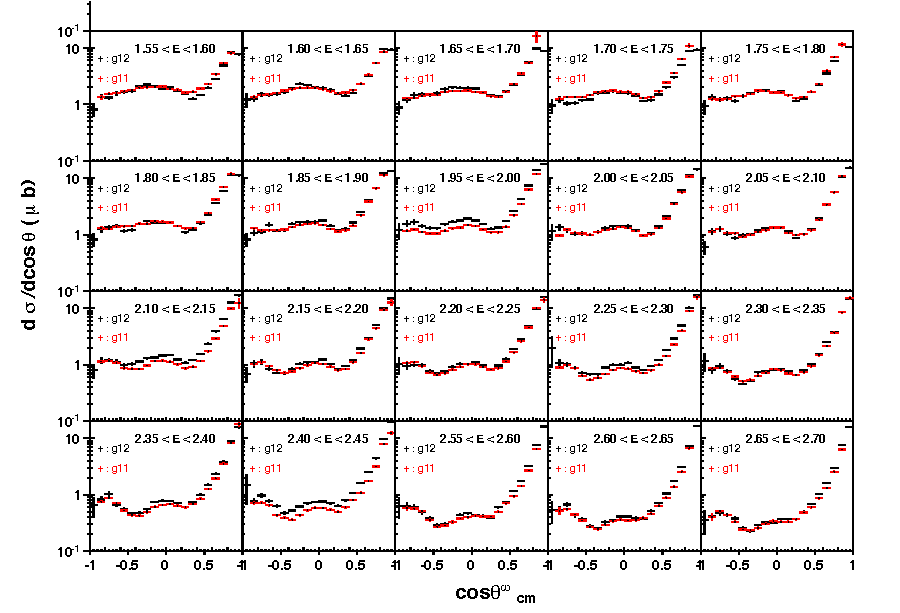
\includegraphics[width=\columnwidth]{{figures/xsec/cross_omega_1}.eps}
\caption[]{\label{fig:xsec.omega1}Differential cross sections for the reaction γ p $\rightarrow$ p ω based on the dominant decay mode ω $\rightarrow$ π$^+$ π$^-$ π$^0$ with a beam energy from 1.5 to 2.5~GeV. Comparison to g11 is in red.}
\end{center}\end{figure}


\begin{figure}[htpb]\begin{center}
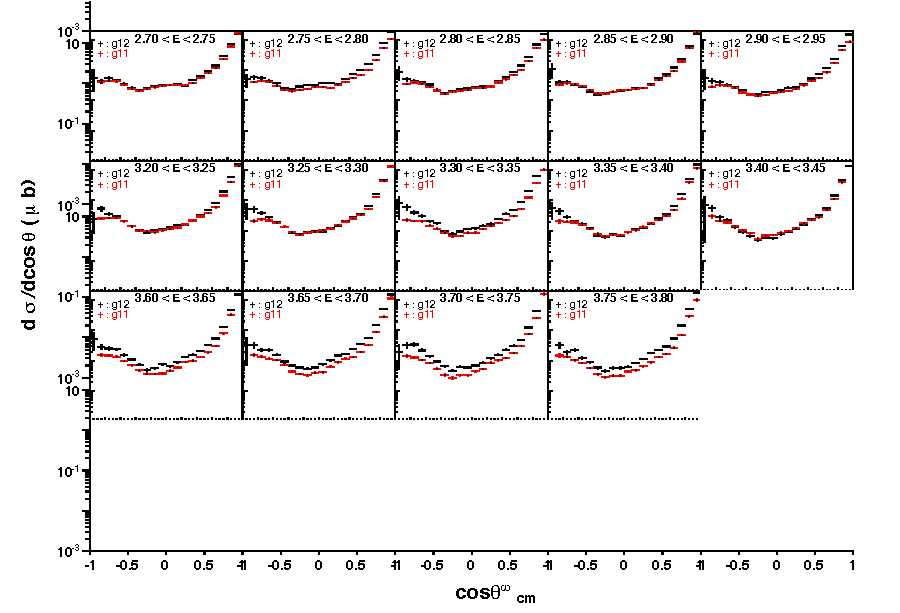
\includegraphics[width=\columnwidth]{{figures/xsec/cross_omega_2}.eps}
\caption[]{\label{fig:xsec.omega2}Differential cross sections for the reaction γ p $\rightarrow$ p ω based on the dominant decay mode ω $\rightarrow$ π$^+$ π$^-$ π$^0$ with a beam energy from 2.5 to 3.65~GeV. Comparison to g11 is in red.}
\end{center}\end{figure}

In terms of the photon multiplicity, at 60-65nA of the production current, about 87$\pm 1$\% of the data has only one photon in the same time bucket chosen for the event, around 12\% has exactly two photons, and approximately 1\% has more than two photons. This has a slight beam energy dependence, however, the variance is on the percent level. The photon multiplicity must be addressed since it is significant. One can correct the cross sections, if  those events with multiple photons are all included in their analyses and the photon was chosen randomly, or they were all excluded. However, one can also address this issue by looping over all photons, and that would not require additional corrections. Since this correction depends on the preference of the individuals, we do not prescribe this as a universal procedure by itself.

The Λ(1115) differential cross section was measured and compared to the \desg{g11a} results shown in Figs.~\ref{fig:lambda.dcs.1} and \ref{fig:lambda.dcs.2}. The \desg{g12} data employed tight timing and fiducial cuts to minimize systematic uncertainty at the expense of larger statistical uncertainty and very low statistics at high energy and large angle.

In this analysis,
\begin{equation}
    \text{γ p} \rightarrow \text{[Λ] Κ$^+$} \rightarrow \text{p π$^-$ K$^+$}
\end{equation}
was simulated with a $t$-slope off the K$^+$ set to unity. The divisions in polar angle were fine enough so that the acceptance was approximately linear in each bin. All three final state particles (p π$^-$ K$^+$) were reconstructed and the trigger was modeled to require two particles to be in two different sectors for the high-energy part of the tagger and three particles in three different sectors for the low-energy part of the tagger. Additionally, the tagger was populated with noise generated from the data using \prog{gpp}'s \verb+-A+ option (see Sec.~\ref{sec:sim.digit}, page~\pageref{cmd:gppAoption}). An associated start counter hit was required for each final-state particle and a timing cut against the \abbr{RF} was set to $\pm 3σ$.

\begin{figure}[htpb]\begin{center}
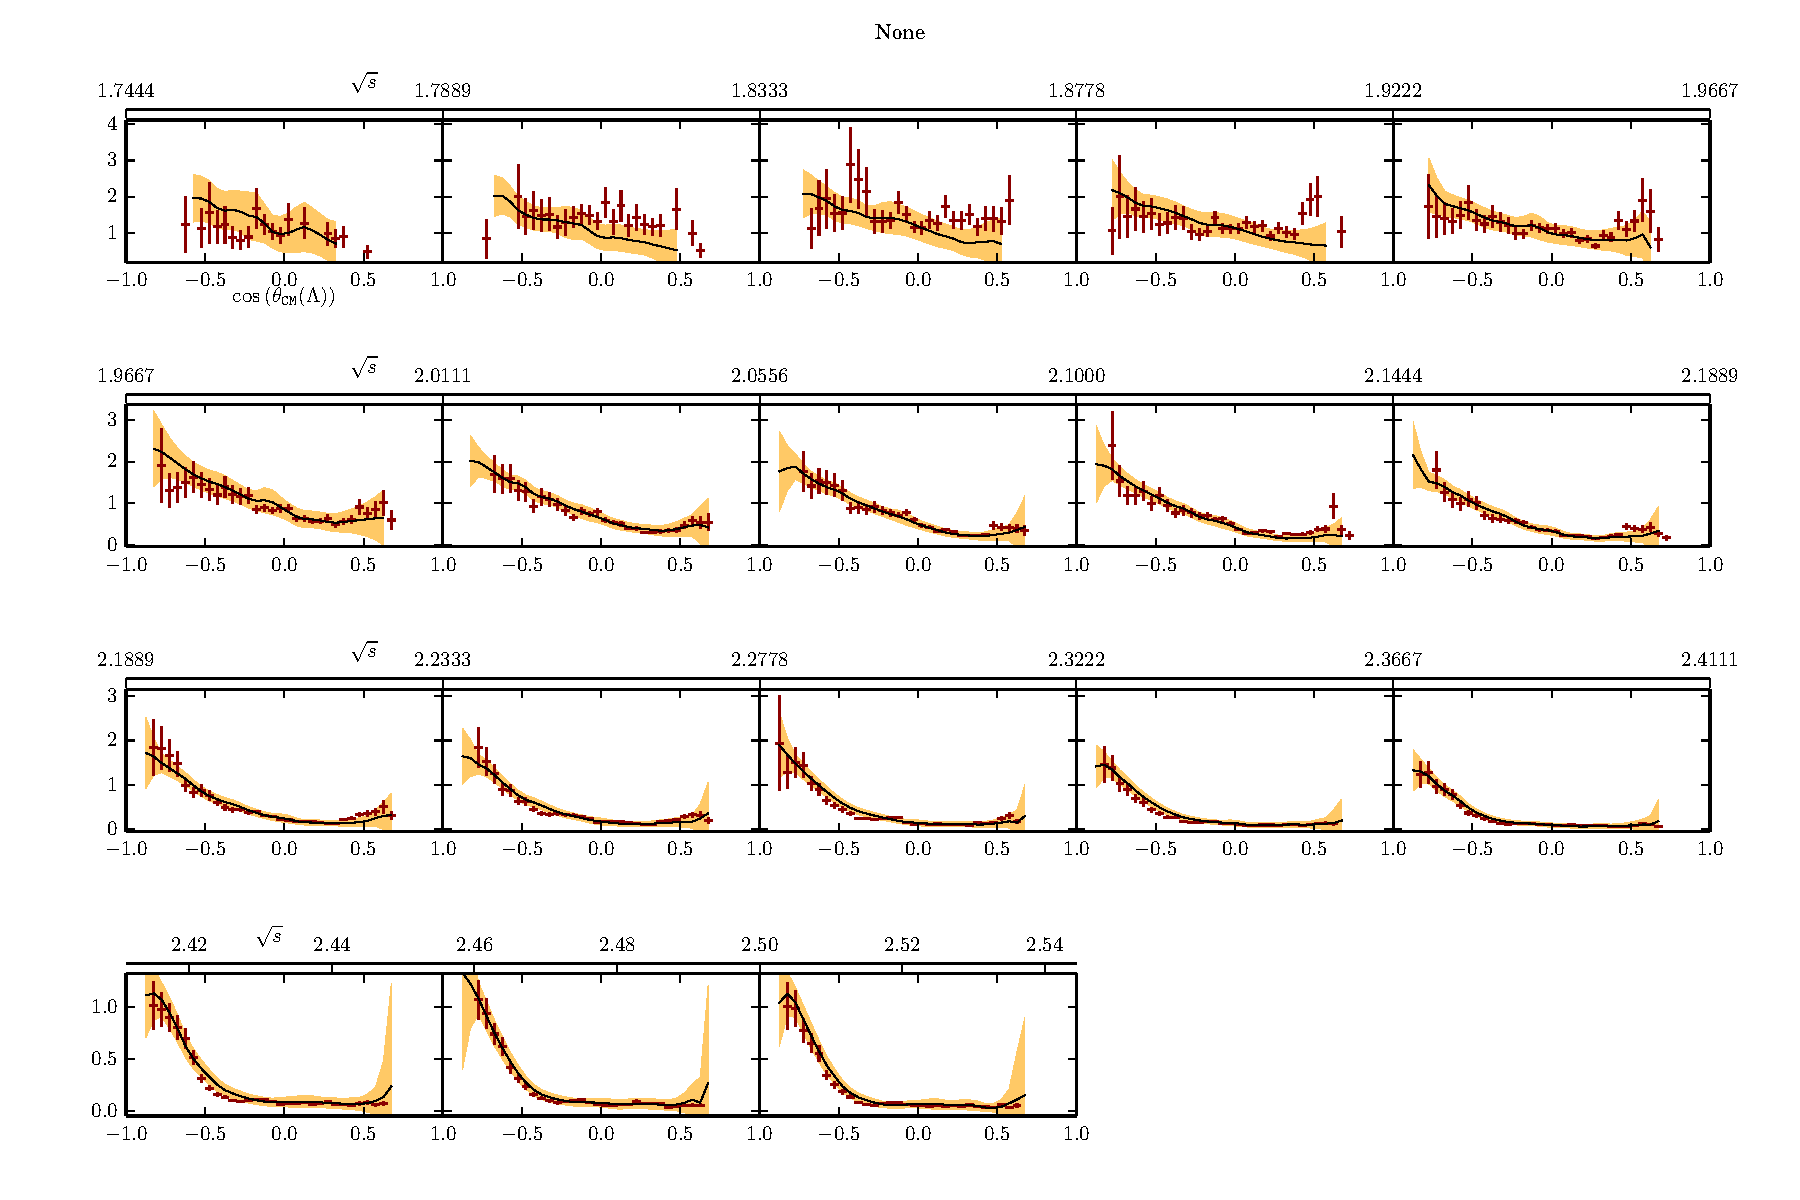
\includegraphics[width=0.99\columnwidth]{{figures/xsec/lambda.dcs.1.linear}.pdf}
\caption[]{\label{fig:lambda.dcs.1}Differential cross section of Λ K$^+$ photoproduction in red with a comparison to \desg{g11a} with the black line and yellow band at $3σ$ of their quoted statistical uncertainty.}
\end{center}\end{figure}


\begin{figure}[htpb]\begin{center}
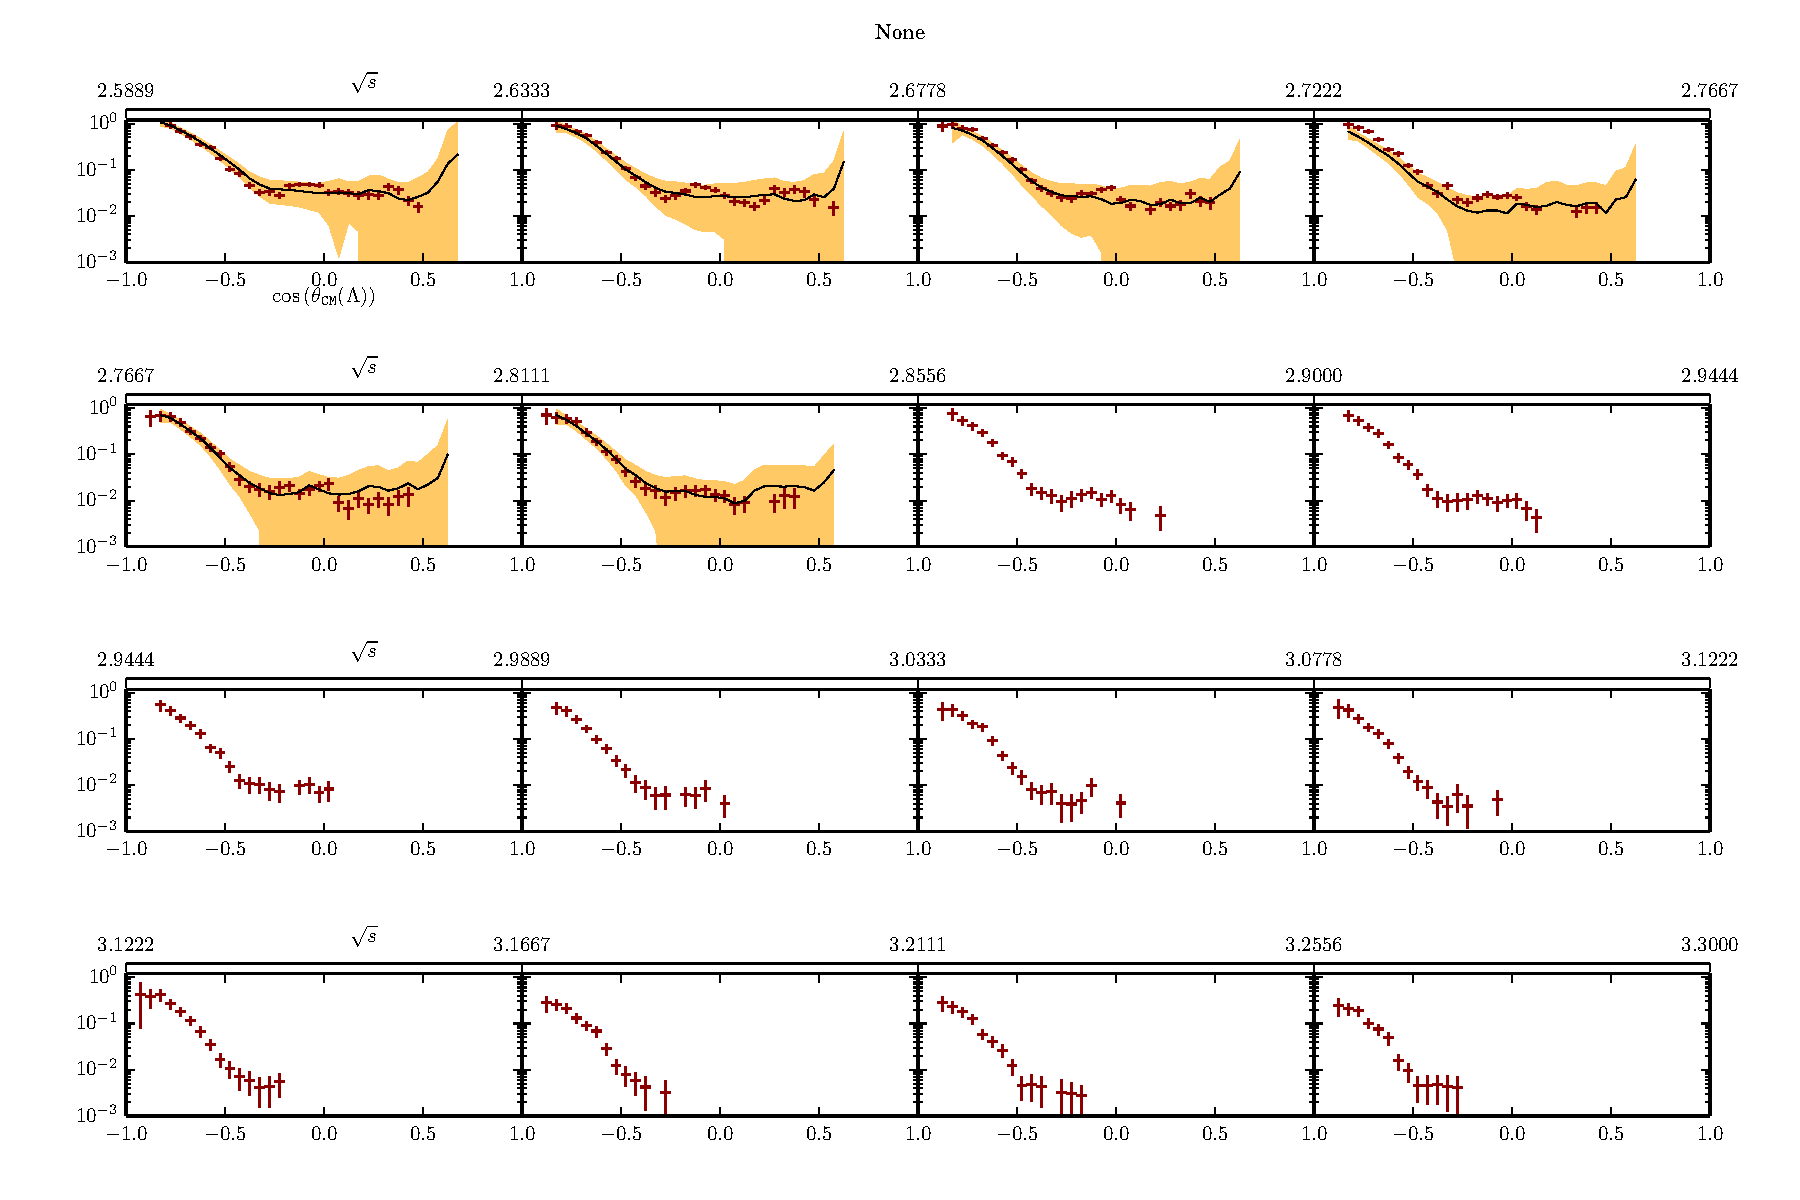
\includegraphics[width=0.99\columnwidth]{{figures/xsec/lambda.dcs.2.log}.pdf}
\caption[]{\label{fig:lambda.dcs.2}Differential cross section of Λ K$^+$ photoproduction in red with a comparison to \desg{g11a} with the black line and yellow band at $3σ$ of their quoted statistical uncertainty.}
\end{center}\end{figure}


The π$^0$ differential cross-section, shown in Figs.~\ref{fig:pi0.xsec.1} and \ref{fig:pi0.xsec.2}, was measured in the reaction
\begin{align}\label{channel}
\text{γ p} \rightarrow \text{p [π$^0$]} \rightarrow \text{p e$^+$ e$^-$ [γ]}
\end{align}
where the detected final state particles were one proton, one positron and one electron, while the final state photon was identified through kinematic fitting. For the identification of the leptons, where the incident photon beam energy was less than 3.6~GeV, the use of the trigger configuration 6 (see Table~\ref{tab:data.trig.conf.2} on page~\pageref{tab:data.trig.conf.2}) was employed. To ensure proper simulation of trigger configuration 6, a trigger model was used which mimicked the discrimination of low voltage from the Cherenkov and Electromagnetic calorimeter PMT's. Simulation was performed using \verb#PLUTO++# to generate phasespace of \ref{channel}. All incident beam photons that were within 2.004~ns of the timed particles were analyzed, meaning if an event had 2 or more incident beam photons that were in time with the detected particles within 2.004~ns, then each photon was analyzed as a separate event along with the quantities of the detected particles.

\begin{figure}[htpb]
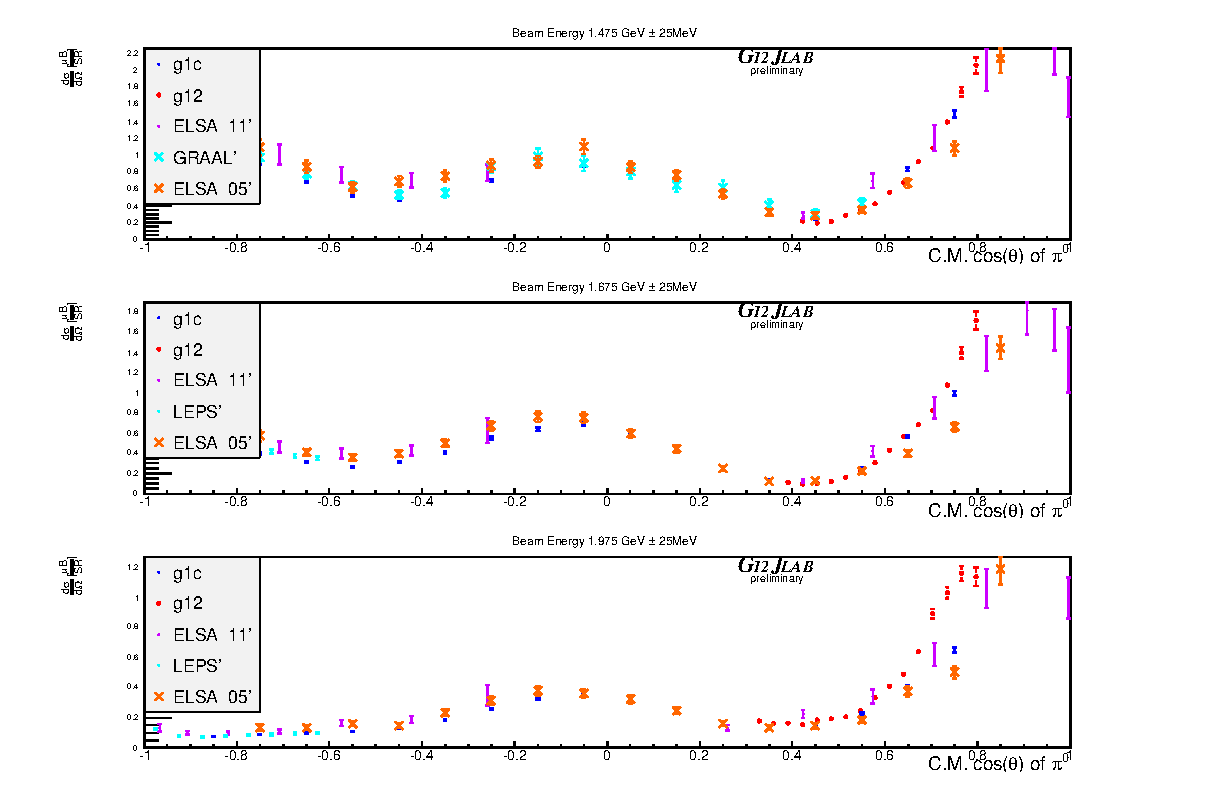
\includegraphics[width=0.95\columnwidth]{figures/xsec/G12_Pi0_XSection_forAnalysisNote_I.eps}
\caption{\label{fig:pi0.xsec.1}Differential cross section of the π$^0$ up to a beam energy of approximately 2~GeV, using the lepton decay channel.}
\end{figure}

\begin{figure}[htpb]
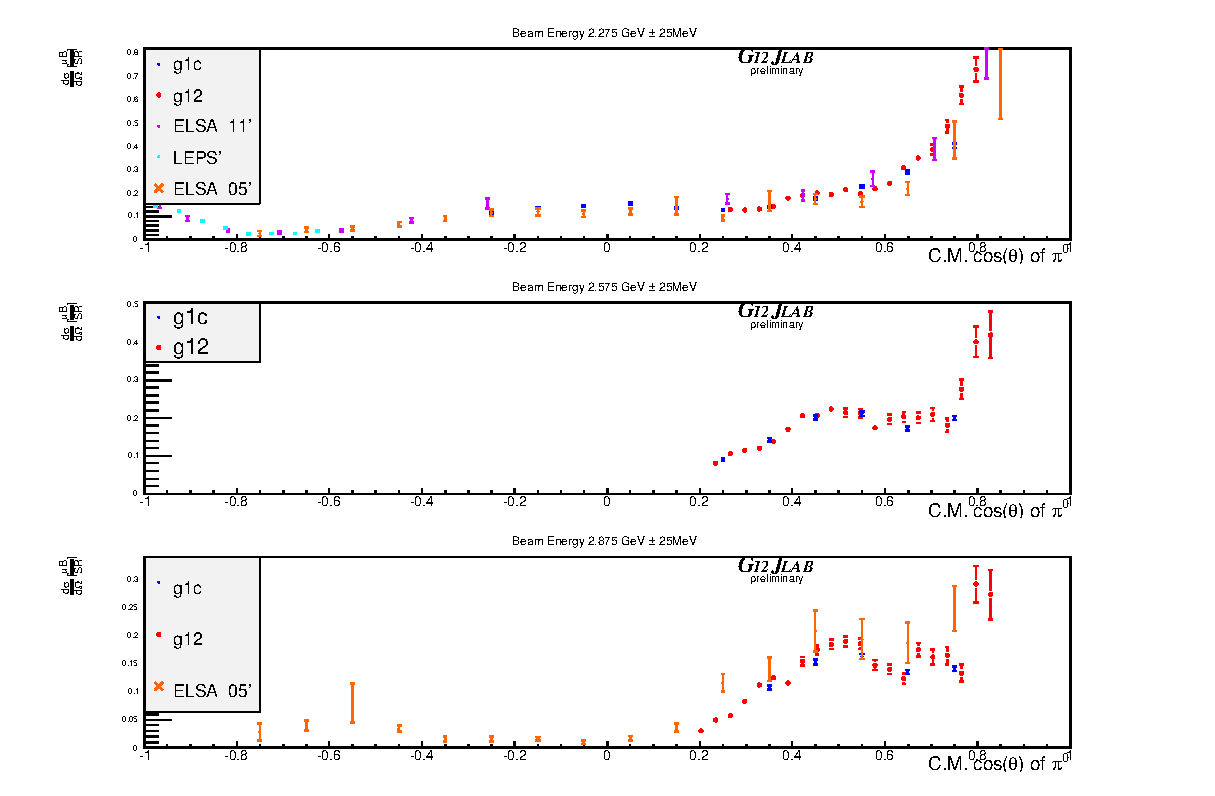
\includegraphics[width=0.95\columnwidth]{figures/xsec/G12_Pi0_XSection_forAnalysisNote_II.eps}
\caption{\label{fig:pi0.xsec.2}Differential cross section of the π$^0$ starting from a beam energy of approximately 2~GeV, using the lepton decay channel.}
\end{figure}

To summarize, the g12 data set does not shown any significant beam-intensity-dependent inefficiency, and the overall normalization, when all corrections documented in this note are applied, can be validated by the consistency between the cross sections such as ω, π$^0$ and Λ when compared with prior results.
